\begin{tikzpicture}[base]
\node[anchor=south west,inner sep=0] (photo) at (0,0) {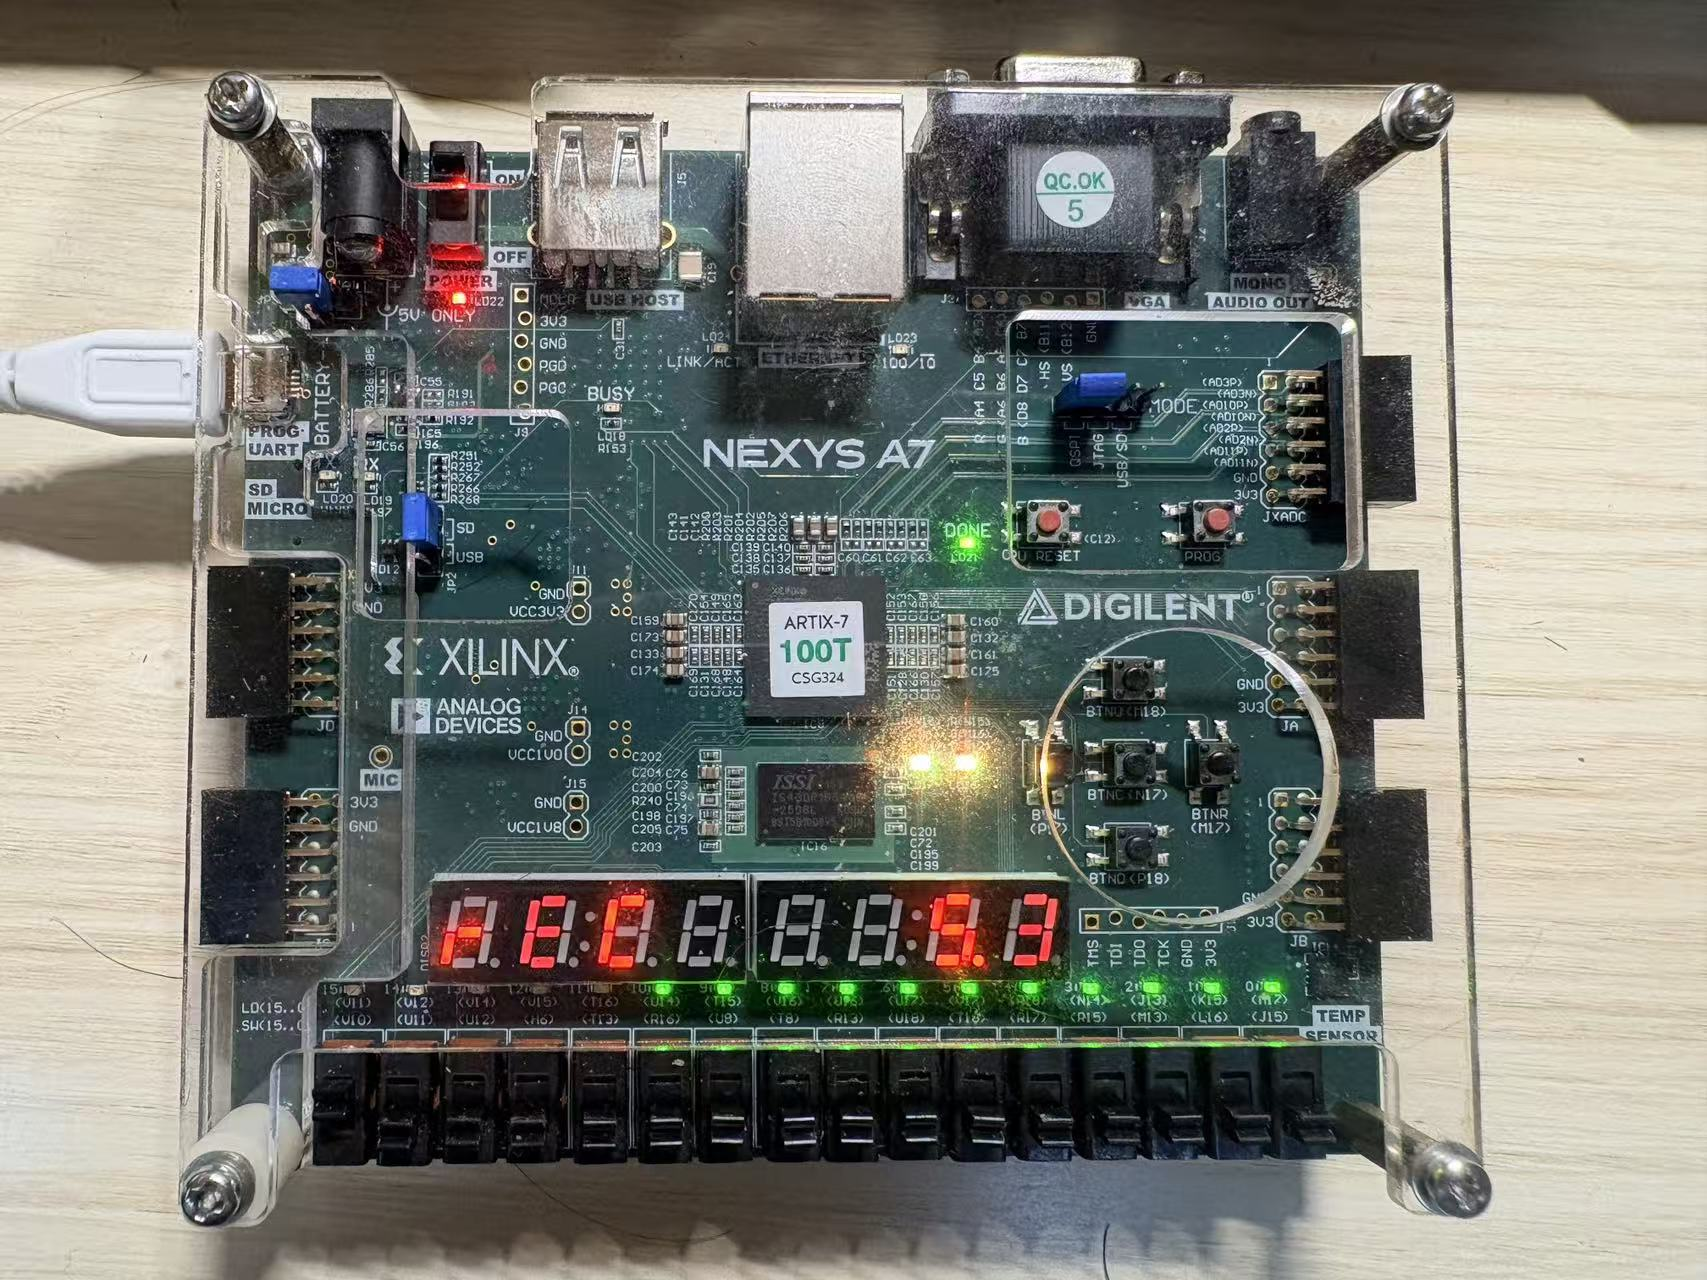
\includegraphics[width=98mm]{figures/board.jpg}};
\begin{scope}[x={(photo.south east)},y={(photo.north west)}]
\node[label,anchor=west] (a) at (1.01,.80) {PROG/UART\\配置与通信};
\node[label,anchor=west] (b) at (1.01,.56) {Artix-7 100T\\采集与处理核心};
\node[label,anchor=west] (c) at (1.01,.32) {数码管 / LED\\任务阶段反馈};
\node[label,anchor=west] (d) at (1.01,.10) {开关与方向键\\模式及交互输入};
\draw[flow,<-] (.12,.69)--++(-.06,0)|-(a.west);
\draw[flow,<-] (.51,.48)--(b.west);
\draw[flow,<-] (.61,.28)--(c.west);
\draw[flow,<-] (.70,.14)--(d.west);
\end{scope}
\end{tikzpicture}
